\scanpage{286}

\[
\begin{aligned}
a{\rho}^{-1}a\rho&\in\widetilde U\rho^{-1}(\tilde u)\\
&\deleted{a\rho^{-1}(a)\in}\\
av^{-1}\rho^{-1}a\rho v&\in\widetilde U\rho^{-1}(\widetilde U)\\
\deleted{av^{-1}a^{-1}}a\rho^{-1}a\rho v&\in\widetilde U(\rho v)^{-1}(\widetilde U)\\
&\widetilde{\deleted{a}}\,\overline{v^{-1}\rho^{-1}\widetilde U}\rho v
\end{aligned}
\]

\[
\begin{aligned}
\rho(a)a&\in\rho(\widetilde U)\widetilde U\\
\rho(ua)a&\in U\\
\deleted{\rho(a)a^{-1}(a)}&\quad\rho(ua)(av)\\
\rho(a)av&\in U_1 U_0\\
&\unsure{\rho(a)|g(a)}
\end{aligned}
\]

% margin note written sideways
\margin{$\mathrm{Et}_{A_0}(s)\cap\mathrm{Et}_{A_0}(\lambda^{-1}t)\ne\varnothing$}

\figure{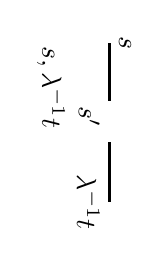
\begin{tikzpicture}[x=0.008cm,y=-0.008cm]
\draw[thick] (0,0)--(0,92);
\draw[thick] (0,157)--(0,252);
\node[above,rotate=-90] at (0,0) {$s$};
\node[below=2mm,rotate=-90] at (0,92) {$s'$};
\node[below,rotate=-90] at (0,252) {$\lambda^{-1}t$};
\node[left,rotate=-90] at (-93,150) {$s,\lambda^{-1}t$};
\end{tikzpicture}}

\[
\rho\qquad\overset{\frown}{U_0\quad U_1}\quad U_\infty
\]

\[
\begin{pmatrix}\lambda&\mu\\0&\lambda^{-1}\end{pmatrix}
\]

\figure{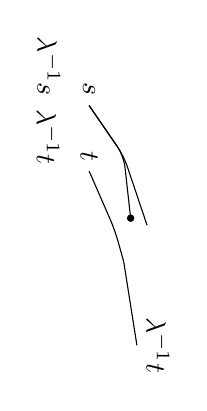
\begin{tikzpicture}[x=0.008cm,y=-0.008cm]
\draw[rounded corners] (0,0)--(55,80)--(66,179);
\draw[rounded corners] (0,0)--(55,80)--(92,190);
\draw[rounded corners] (0,104)--(41,198)--(55,248);
\draw (55,248)--(76,381);
\fill (66,179) circle[radius=1.35pt];
\node[left,rotate=-90] at (0,0) {$s$};
\node[left,rotate=-90] at (0,104) {$t$};
\node[left,rotate=-90] at (-64,0) {$\lambda^{-1}s$};
\node[left,rotate=-90] at (-65,110) {$\lambda^{-1}t$};
\node[above,rotate=-90] at (76,381) {$\lambda^{-1}t$};
\end{tikzpicture}}

\[
\begin{aligned}
\varepsilon_0=\sigma_\infty^{-1}\rho\qquad
\sigma_\infty(\varepsilon_0)&=\rho\,\sigma_\infty\\
\unsure{\rho_\infty|\rho}(\varepsilon_0)&=\rho\,\sigma_\infty^{-1}
\end{aligned}\ \bigg|\ \text{\unsure{définis|diffèrent} \unsure{par un|pour|par $\omega$}}
\]

\[
\begin{aligned}
\rho:\quad e_1&\longmapsto-e_2\\
\deleted{\unsure{e_1|e_\tau}}\!:\quad e_2&\longmapsto e_1+e_2\\
&\omega
\end{aligned}
\]

\figure{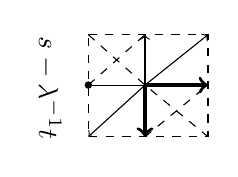
\begin{tikzpicture}[x=0.008cm,y=-0.008cm]
\draw[dashed] (0,0)--(90,0)--(190,0)--(190,80)--(190,162)--(90,162)--(0,162)--(0,80)--(0,0);
\draw[dashed] (0,0)--(90,80)--(190,162);
\draw[dashed] (0,80)--(90,0);
\draw[dashed] (90,162)--(190,80);
\draw[->] (90,80)--(90,0);
\draw[->] (90,80)--(190,0);
\draw[very thick,->] (90,80)--(190,80);
\draw[very thick,->] (90,80)--(90,162);
\draw[->] (90,80)--(0,162);
\draw (0,80)--(90,80);
\fill (0,80) circle[radius=1.35pt];
\node[rotate=-90] at (-62,85) {$s-\lambda^{-1}t$};
\end{tikzpicture}}

\[
\lambda^{-1}s=s\qquad\deleted{\unsure{s=s}}\qquad\deleted{\lambda^{-1}s=t}
\]

\figure{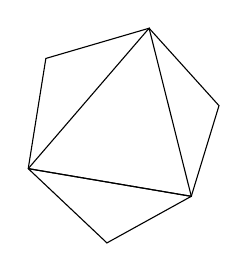
\begin{tikzpicture}[x=0.008cm,y=-0.008cm]
\draw (28,48)--(192,0)--(303,123)--(259,267)--(125,341)--(0,223)--cycle;
\draw (0,223)--(192,0)--(259,267)--(0,223);
\draw[thin] (0,223)--(259,267);
\end{tikzpicture}}

\[
\begin{pmatrix}1&0\\\mu&1\end{pmatrix}\begin{pmatrix}1&\mu'\\0&1\end{pmatrix}=\begin{pmatrix}1&\mu'\\\mu&1+\mu\mu'\end{pmatrix}
\]

\figure{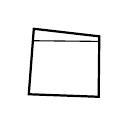
\begin{tikzpicture}[x=0.008cm,y=-0.008cm]
\draw[thick] (0,0)--(104,12)--(103,108)--(-8,104)--cycle;
\draw (-1,19)--(102,20);
\end{tikzpicture}}

% margin note written sideways
\margin{$E_0\quad E_0$}

\[
\rho=\begin{pmatrix}0&1\\-1&1\end{pmatrix}
\]

\[
\begin{aligned}
\underbrace{\begin{pmatrix}0&1\\-1&1\end{pmatrix}\begin{pmatrix}\lambda&0\\0&\lambda'\end{pmatrix}}\,
\underbrace{\begin{pmatrix}1&-1\\1&0\end{pmatrix}\begin{pmatrix}\lambda&0\\0&\lambda'\end{pmatrix}}
&=\begin{pmatrix}\lambda\lambda'&0\\\lambda\lambda'-\lambda^2&\lambda\lambda'\end{pmatrix}\\
\begin{pmatrix}0&\lambda'\\-\lambda&\lambda'\end{pmatrix}\begin{pmatrix}\lambda&-\lambda'\\\lambda&0\end{pmatrix}&=\begin{pmatrix}1&0\\1-\lambda^2&1\end{pmatrix}
\end{aligned}
\]

\[
\begin{aligned}\deleted{\mu=}\qquad\mu'&=0\\ \mu&=1-\lambda^{\unsure{2|\sim}}\end{aligned}
\]

\figure{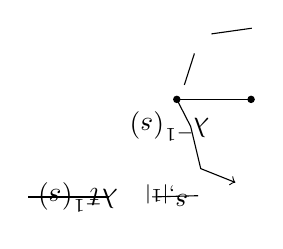
\begin{tikzpicture}[x=0.008cm,y=-0.008cm]
\draw (0,0)--(128,0);
\draw (197,0)--(270,-2);
\draw[->] (236,-155)--(258,-112)--(274,-45)--(329,-23);
\draw (236,-155)--(354,-155);
\draw (248,-178)--(264,-228);
\draw (291,-259)--(355,-268);
\fill (236,-155) circle[radius=1.35pt];
\fill (354,-155) circle[radius=1.35pt];
\node[left,rotate=180] at (0,0) {$\lambda^{-1}(s)$};
\node[right,rotate=180] at (128,0) {$t$};
\node[right,rotate=180] at (270,-2) {$s_{\unsure{,|1|{}}}$};
\node[left=9mm,rotate=180] at (258,-112) {$\lambda^{-1}(s)$};
\end{tikzpicture}}

% archive sheet number: 285
